\cleardoublepage
\phantomsection
\chapter{Functions \& Methods}

\begin{quote}
\textit{Either mathematics is too big for the human mind, or the human mind is
more than a machine.} --- Kurt Gödel
\end{quote}

In this chapter, we are going to learn more about functions.  You have
already seen functions in previous chapters.  Functions provide a way
to group statements together and call it multiple times.  If you don't
use functions, the same statements will be written again and again in
different parts of your code.  Ultimately functions helps you to reuse
code.  A function can optionally accept arguments and execute
statements and optionally return values.

Mathematical function would be a good analogy to understand the
concept of functions in programming.  We have seen this mathematical
function in the Quickstart chapter.

\begin{figure}[h!]
\centering
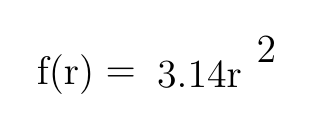
\begin{tikzpicture}
\node at (1.7,0) {{\Large 3.14r}};
\node at (2.55,0.32) {{\Large 2}};
\node at (0,0) {{\Large f(r)}};
\node at (0.7,0) {{\Large =}};
\end{tikzpicture}
\caption{Mathematical function for area of a circle}
\end{figure}

This function square the input value and multiply with 3.14.
Depending on the input value the output varies.

\begin{figure}[h!]
\centering
\begin{tikzpicture}
\draw [thick, ->] (0,1) -- (2,1);
\node at (.5,1.2) {r};
\draw [thick] (2,0) rectangle (7,2);
\node at (4.5,1) {3.14r};
\node at (5.1,1.2) {2};
\node at (4.5,2.3) {f(r)};
\draw [thick, ->] (7,1) -- (9,1);
\node at (8.5,1.2) {y};
\end{tikzpicture}
\caption{Blackbox representation of a function}
\end{figure}

As you can see in the diagram, \texttt{r} is the input and \texttt{y}
is the output.  A function in Go can take input arguments and perform
actions and return values.  A minimal implementation of this function
in Go looks like this.

\begin{lstlisting}[numbers=none]
func Area(r float64) float64 {
    return 3.14 * r * r
}
\end{lstlisting}

The function declaration starts with \texttt{func} keyword.  In the
above example, \texttt{Area} is the function name which can be later
used to call the function.  The arguments that can be received by this
function is given within brackets.  After the input parameters you can
specify the output parameters.  If there are more than one output
parameter required, use a bracket around that.  After the output
parameters, add one opening curly bracket.  The statements can be
written in the next line on wards until the closing curly bracket.  It
is recommended to start a new line after the opening curly bracket and
closing bracket can be in a line by its own.

Here is a complete example with usage of the Area function.

\begin{lstlisting}[caption=Function to calculate area of circle (area.go)]
package main

import "fmt"

func Area(r float64) float64 {
    return 3.14 * r * r
}

func main() {
    area := Area(5.0)
    fmt.Println(area)
}
\end{lstlisting}

In the above example, the \texttt{Area} function is called with
argument value as \texttt{5.0} (line number 10).  And the short
variable declaration syntax is used to assign value returned by the
function.  The type of the variable \texttt{area} will be
\texttt{float64} as the \texttt{Area} function returns with that type.

If you run the above program, you will get the output like this:

\begin{lstlisting}[numbers=none]
$ go run area.go
78.5
\end{lstlisting}

\section{Parameters}

A function can accept any number of arguments depending on the
parameters defined.  The \texttt{Area} function in the previous
section accepts one argument.

If the function definition doesn't have any parameters, you cannot
pass any arguments.  Parameter\index{parameter} is the variable used
in the declaration of a function.  Where as
argument\index{parameter!argument} is the actual value of this
variable that gets passed to function.  Consider this example:

\begin{lstlisting}[caption=Function without any parameters]
package main

import (
     "fmt"
     "time"
)

func TimeNow() string {
     t := time.Now()
     h := t.Hour()
     m := t.Minute()
     return fmt.Sprintf("%d:%d", h, m)
}

func main() {
     now := TimeNow()
     fmt.Println(now)
}
\end{lstlisting}

The \texttt{TimeNow} function doesn't declare any parameters.  So,
when the function is called, no arguments are passed.  If you try to
pass any arguments, you will get an error with this
message: \texttt{too many arguments in call to TimeNow}.

\subsection{More parameters}

A function can accepts more arguments of same or different types.

\begin{lstlisting}[caption=Function with two parameters]
package main

import "fmt"

func sum(a int, b int) int {
    return a + b
}

func main() {
    s := sum(5, 2)
    fmt.Println(s)
}
\end{lstlisting}

The above \texttt{sum} function accepts two integer parameters.  Since
both parameters are integers, the type can be specified once.

\begin{lstlisting}[numbers=none]
func sum(a, b int) int {
    return a + b
}
\end{lstlisting}

\section{Return Values}

A function can return any number of values\index{return}.  The calling
side should have comma separated variables to receive the return
values.  If you are only interested in a particular return value, you
can use underscore as the variable name for others.

Here is an example function which return two values:

\begin{lstlisting}[caption=Function with two return values]
package main

import "fmt"

func div(a, b int) (int, int) {
    return a / b, a % b
}

func main() {
    v, r := div(5, 2)
    fmt.Println(v, r)
}
\end{lstlisting}

In the above example, the div function return two values.  So two
variables are used to assign the values.  If you use one variable it
will produce compile time error.  The compile time error will be
produced, if more than two variables are used to assigned.  However,
it is possible to call the function without assigning to any
variables.

\begin{lstlisting}[numbers=none]
v, _ := div(5, 2)
div(5, 2)
\end{lstlisting}

By convention, the last return value will be an error value.  Here is
a modified example.

\begin{lstlisting}[numbers=none]
func div(a, b int) (int, int, error) {
    if b == 0 {
        err := errors.New("Zero division error")
        return 0, 0, err
    }
    return a / b, a % b, nil
}
\end{lstlisting}

In the above example, package \texttt{errors} is used to create a new
error value.  If there is no error, a \texttt{nil} value can be
returned.

\subsection{Named output parameters}

It is possible to specify name for output
parameters\index{return!named parameter}.  These variables can be used
to assign values.  With named output parameters, return statement need
not to explicitly specify the variables.

\begin{lstlisting}[caption=Function with named output parameters]
package main

import "fmt"

func div(a, b int) (int d, int r) {
    d := a / b
    r := a % b
    return
}

func main() {
    v, r := div(5, 2)
    fmt.Println(v, r)
}
\end{lstlisting}

\section{Variadic Functions}

A function\index{function!variadic}\index{variadic function} which can
receive any number of arguments of a particular type is called
variadic function.  Variable name along with an ellipsis
(\texttt{...}) symbol is used to declare variadic parameters.
The \texttt{fmt.Println} is a commonly used variadic function.

Here is a complete example:

\begin{lstlisting}[caption=Variadic Function (variadic.go)]
package main

import "fmt"

func sum(nums ...int) {
    fmt.Printf("%#v ", nums)
    total := 0
    for _, num := range nums {
        total += num
    }
    fmt.Println(total)
}

func main() {
    sum(1, 2)
    sum(1, 2, 3)
    nums := []int{1, 2, 3, 4}
    sum(nums...)
}
\end{lstlisting}

If you run the above program, this will be the output:

\begin{lstlisting}[numbers=none]
$ go run variadic.go
[]int{1, 2} Sum: 3
[]int{1, 2, 3} Sum: 6
[]int{1, 2, 3, 4} Sum: 10
\end{lstlisting}

As you can see the arguments are captured into a slice.  You can send
values in a slice to a variadic function using the ellipsis syntax as
a suffix.

\section{Anonymous Functions}

It is possible to declare a function without a
name\index{function!anonymous}.  These type of functions can be used
to create function closures.  A closure is an anonymous function that
access variables from outside its body.

\begin{lstlisting}[caption=Anonymous Function (anonfunc.go)]
package main

import "fmt"

func main() {
     name := "Tom"
     func() {
            fmt.Println("Hello", name)
     }()
}
\end{lstlisting}

\section{Function as Value}

Function is a first class citizen\index{function!value} in Go, so it
can be passed as an argument and return as a value.

\begin{lstlisting}[caption=Function as value (funcvalue.go)]
package main

import "fmt"

func Greeting(msg string) func(name string) string {
}

func main() {
     name := "Tom"
     func() {
            fmt.Println("Hello", name)
     }()
}
\end{lstlisting}

\section{Methods}
\label{sec:methods}

A function can be associated with a type, that is called method.
Additional methods can be added to types defined locally.  However,
adding additional methods for non-local type is not allowed.  Here is
an example program:

\begin{lstlisting}[numbers=none]
package main

import (
        "fmt"
        "os"
        "strconv"
)

type Number int

func (num Number) Even() bool {
        if num%2 == 0 {
                return true
        } else {
                return false
        }

}

func main() {
        i := os.Args[1]
        n, err := strconv.Atoi(i)
        if err != nil {
                fmt.Println("Not a number:", i)
                os.Exit(1)
        }
        num := Number(n)
        fmt.Println(num.Even())
}
\end{lstlisting}

In the above program, a custom type named \texttt{Number} is
defined. Later a method named \texttt{Even} is defined below.  To
define a method for any type, the syntax is like this: \texttt{func
  (value CustomType) MethodName()}.  You can also define input
parameters and output parameters.  In the above the output parameter
is given as a \texttt{bool} value.

You can associate methods\index{method} to structs. Consider this
struct:

\begin{lstlisting}[numbers=none]
type Rectangle struct {
    Width  float64
    Height float64
}
\end{lstlisting}

If you want methods to calculate area and perimeter for this rectangle,
you can define methods like this:

\begin{lstlisting}[numbers=none]
func (r Rectangle) Area() float64 {
    return r.Width * r.Height
}

func (r Rectangle) Perimeter() float64 {
    return 2 * (r.Width * r.Height)
}
\end{lstlisting}

You can call these methods from the struct initialized using
the \texttt{Rectangle} struct.  Here is an example:

\begin{lstlisting}[numbers=none]
r := Rectangle{3.0, 5.0}
area := r.Area()
perimeter := r.Perimeter()
\end{lstlisting}

When a function is bound to a type, it is called method\index{method}.
The type that is bound is called receiver.  A receiver could be any
type with a name.  When you declare a method, it is defined using
receiver argument.  The receiver argument points to the type where the
method will be available.  The receiver argument is specified between
func keyword and the method name inside a bracket with a name.

Methods can be defined only on types declared in the same package.
Declaring a method on built-in type is also illegal.

Here is an example:

\begin{lstlisting}[caption=Method]
package main

import "fmt"

type Circle struct {
    radius float64
}

func (c Circle) Area() float64 {
    return 3.14 * c.radius * c.radius
}

func main() {
     c := Circle{3.4}
     a := c.Area()
     fmt.Println(a)
}
\end{lstlisting}


In the above example, the method \texttt{Area} calculate area for a
circle.

The receiver could be pointer also.  Here is a modified example with
pointer receiver:

\lstinputlisting[caption=Method with pointer receiver]{code/functions/pointer1.go}

In the above example, the \texttt{Area} method is using a pointer
receiver.  When creating object, you can create a normal value or a
pointer value.  Calling the \texttt{Area} can use either a normal
value or a pointer value.

Pointer receiver\index{pointer!receiver} can be used when for any of
these three reason:

\begin{itemize}
\item To modify the receiver itself by changing the value of attributes.
\item The object is very large and a passing a deep copy is expensive.
\item Consistency: Let all methods have pointer receivers.
\end{itemize}

You can use new function to allocate memory for \textit{struct}:

\begin{lstlisting}[numbers=none]
type Temperature struct{
     Value float64
}

name := new(Temperature)
\end{lstlisting}

In the above example, the zero value is allocated and assigned to the
variable \texttt{name}.  But in some cases, zero value is not what you
required.  So you can use \texttt{\&} to with struct syntax like this:

\begin{lstlisting}[numbers=none]
type Temperature struct{
     Value float64
}

name := &Temperature{Value: -7.6}
\end{lstlisting}

As you can see, the temperature value is set to \texttt{-7.6} and
assigned to the variable.

\section{Exercises}

\textbf{Exercise 1:} Write a method to calculate the area of a rectangle.

\textbf{Solution:}

\begin{lstlisting}[numbers=none]
type Rectangle struct {
    Width  float64
    Height float64
}

func (r Rectangle) Area() float64 {
    return r.Width * r.Height
}
\end{lstlisting}

\subsection{Additional Exercises}

Answers to these additional exercises are given in the Appendix A.

\textbf{Problem 1:} Write a program with a function to calculate perimeter of a circle.

\section*{Summary}

This chapter explained all the major aspects of functions in Go.  The
chapter covered how to send input parameters and return values.  It
also explained about variadic function and anonymous function.  This
chapter briefly also covered methods.  The next chapter will cover
interfaces.  Along with that, we will learn more about methods.
